%% Informe de avance de la Etapa 2 del trabajo de titulo (entrega del 2 de
%% octubre de 2026). Documento autocontenido en un solo archivo, por decision
%% del profesor guia: contiene solo los avances de esta etapa, sin repetir lo
%% entregado en la Etapa 1.
%%
%% Vive en la carpeta informe/ para usar el mismo logo (images/) y el mismo
%% referencias.bib que el documento general. En Overleaf se compila eligiendo
%% este archivo en Menu > Main document.
%%
%% El capitulo 2 y el anexo son copia de cap2.tex y de la seccion del
%% contrato de datos de anexos.tex en el commit 0377d0b, con dos ajustes: la
%% referencia al capitulo 1 apunta al cuadro de tramos de este informe y las
%% secciones 2.5 y 2.6 declaran que se desarrollan en el sprint 3. Desde ahora
%% los cambios de diseno se hacen aqui y se llevan a cap2.tex al integrar este
%% informe al documento general.

\documentclass[12pt,oneside,spanish,oldfontcommands]{memoir}

% --- Bibliografia ---
\usepackage[backend=biber,style=apa]{biblatex}
\addbibresource{referencias.bib}
\DeclareLanguageMapping{spanish}{spanish-apa}

% --- Fuentes e idioma ---
\usepackage{mathpazo}
\usepackage[T1]{fontenc}
\usepackage[utf8]{inputenc}
\usepackage{babel}
\addto\shorthandsspanish{\spanishdeactivate{~<>.}}
\usepackage[none]{hyphenat}

% Detector de tildes mal codificadas: si ves una fila de asteriscos en el
% PDF, ese texto viene con acentos descompuestos y hay que retipearlo.
\DeclareUnicodeCharacter{0301}{*************************************}

% --- Estructura ---
\setcounter{secnumdepth}{3}
\setcounter{tocdepth}{3}
\setlength{\parskip}{\medskipamount}
\setlength{\parindent}{0pt}

% --- Tablas y figuras ---
\usepackage{array}
\usepackage{booktabs}
\usepackage{longtable}
\usepackage{multirow}
\usepackage{float}
\usepackage{graphicx}
\usepackage{tikz}
\usetikzlibrary{positioning,fit,arrows.meta,calc}

% --- Algoritmos ---
\usepackage{algorithm}
\usepackage{algorithmicx}
\usepackage{algpseudocode}
\makeatletter
\renewcommand{\ALG@name}{Algoritmo}
\makeatother

% --- Varios ---
\usepackage{textcomp}
\usepackage{csquotes}
\usepackage{url}
\usepackage{hyperref}

\providecommand{\definitionname}{Definición}
\providecommand{\theoremname}{Teorema}

\begin{document}

\sloppy

% ---------------- Portada ----------------
\vspace*{-6\baselineskip}
\pagenumbering{gobble}
\hspace*{-0.0\textwidth}
\includegraphics[width=\textwidth]{images/Logo_depto_ing_informatica.png}\nonumber

\vspace{3cm}

\begin{center}
    \textbf{DESARROLLO DE UN ALGORITMO DE IDENTIFICACIÓN DE EVENTOS
    SISMO-VOLCÁNICOS MEDIANTE DETECCIÓN AUTOMÁTICA Y CLASIFICACIÓN CON CNN}
\end{center}
\vspace{3.5cm}

\begin{center}
por
\par\end{center}

\begin{center}
Patricio Valdés Troncoso\vspace{3cm}
\par\end{center}

\begin{center}
Informe de avance del Trabajo de Título, Etapa 2\\
Facultad de Ingeniería de la Universidad Católica de Temuco\\
Profesor guía: Ricardo Soto
\par\end{center}
\begin{center}
- Temuco, Octubre 2026 -
\par\end{center}

\clearpage
\pagenumbering{roman}

\tableofcontents{}
\pagebreak{}

\listoffigures
\pagebreak{}

\listoftables
\pagebreak{}

% ---------------- Cuerpo ----------------
\pagenumbering{arabic}
\setcounter{page}{1}

% ======================================================================
% CAPITULO 1. Incorporacion de la retroalimentacion (rubrica: 20 %)
% ======================================================================
\chapter{Incorporación de la retroalimentación}
\label{cap:retroalimentacion}

Este informe reúne los avances de la Etapa 2 del trabajo de título. Por
decisión del profesor guía se entrega como un documento aparte, centrado en lo
que corresponde a esta etapa: el problema, el estado del arte, los
requerimientos y la planificación se entregaron en la Etapa 1 y no se repiten.
Los códigos de hallazgos (E1 a E9), requerimientos (RF y RNF), alternativas (D1
a D7), criterios de aceptación (CA) y tareas del backlog (B) remiten a ese
documento. Al cierre del trabajo integraré este informe al documento general de
la tesis.

Este capítulo registra la retroalimentación recibida desde la Etapa 1 y cómo la
incorporé. El Capítulo~\ref{cap:diseno} presenta el diseño del sistema, que es
el foco de la etapa; el Capítulo~\ref{cap:detectores}, la estrategia y los
resultados de los detectores, y el Capítulo~\ref{cap:registro}, el avance del
backlog y sus desviaciones.

\section{Objetivos reformulados}
\label{sec:objetivos-reformulados}

El 15 de septiembre de 2026 el profesor guía reescribió los objetivos del
trabajo. Los adopto textualmente:

\begin{quote}
\textbf{Objetivo general.} Desarrollar un sistema de identificación de eventos
sismovolcánicos del Complejo Volcánico Nevados de Chillán, basado en la
detección automática y la posterior clasificación de los eventos recortados a
partir de sus espectrogramas mediante una red neuronal convolucional ajustada
por transferencia de aprendizaje.

\textbf{OE1.} Evaluar el desempeño de STA/LTA, EQTransformer y PhaseNet en la
detección de eventos sobre registros continuos etiquetados del Complejo
Volcánico Nevados de Chillán, considerando la sensibilidad, la tasa de falsos
positivos y la calidad de los recortes mediante la intersección sobre unión
(IoU).

\textbf{OE2.} Implementar un procedimiento de generación de espectrogramas a
partir de los eventos identificados por los detectores, que considere la
variabilidad de su duración, los errores de delimitación temporal y el
solapamiento entre eventos.

\textbf{OE3.} Ajustar mediante transferencia de aprendizaje una red neuronal
convolucional para clasificar los espectrogramas en eventos VT, LP, TR y una
categoría de rechazo, utilizando un protocolo de entrenamiento y evaluación
reproducible.

\textbf{OE4.} Evaluar el sistema integrado sobre registros continuos,
comparando el desempeño de la clasificación con recortes de referencia y
recortes automáticos, y reportando los resultados por clase y el tiempo de
procesamiento.
\end{quote}

Frente a la Etapa 1 hay tres cambios de fondo. El objetivo general fija que la
clasificación se hará a partir de espectrogramas, con una red ajustada por
transferencia de aprendizaje. OE3 deja de comparar tres arquitecturas y pasa a
ajustar una sola. La evaluación del sistema integrado se separa en un cuarto
objetivo, OE4. La plantilla del trabajo de título recomienda no superar tres
objetivos específicos; en la reunión del 21 de septiembre el profesor guía
decidió mantener los cuatro. El Cuadro~\ref{tab:cambios-15sep} resume los
cambios que la reformulación produjo en el resto del proyecto.

{\small
\begin{longtable}{>{\raggedright\arraybackslash}p{4.8cm}>{\raggedright\arraybackslash}p{3.4cm}>{\raggedright\arraybackslash}p{3.1cm}}
\caption{Cambios derivados de la reformulación de los objetivos del 15 de septiembre de 2026.}\label{tab:cambios-15sep}\\
\toprule
\textbf{Cambio} & \textbf{Origen} & \textbf{Dónde se refleja} \\
\midrule
\endfirsthead
\multicolumn{3}{l}{\itshape Cuadro \thetable{} (continuación)}\\
\toprule
\textbf{Cambio} & \textbf{Origen} & \textbf{Dónde se refleja} \\
\midrule
\endhead
\midrule
\multicolumn{3}{r}{\itshape Continúa en la página siguiente}\\
\endfoot
\bottomrule
\endlastfoot
Objetivo general y objetivos específicos reformulados; pasan de tres a cuatro &
Correo del profesor guía, 15 de septiembre &
Sección~\ref{sec:objetivos-reformulados}; capítulo 1 y anexo de criterios SMART
del documento general \\
\addlinespace
D5 deja de comparar tres arquitecturas y pasa a decidir la estrategia de
entrenamiento: transferencia desde ImageNet sobre una sola CNN, la VGG16 &
Consecuencia de OE3 &
Sección~\ref{sec:clasificador-transferencia}; evaluación de alternativas del
documento general \\
\addlinespace
RF-17, CA-04 y HU-09 se reescriben en términos de ajuste por transferencia;
B-23 y B-24 se funden en una sola tarea B-23 de 10~h, y el identificador B-24 se
retira sin reutilizarse &
Consecuencia de OE3 &
Capítulo~\ref{cap:registro}; anexos de requerimientos, aceptación y backlog del
documento general \\
\addlinespace
La evaluación integrada pasa a OE4: RF-18 a RF-20 y la épica EP-5 responden a
OE4, y B-25, que mide el tiempo de procesamiento, sube de \emph{Debería} a
\emph{Debe} &
Consecuencia de OE4 &
Sección~\ref{sec:protocolo-evaluacion}; Capítulo~\ref{cap:registro} \\
\addlinespace
El backlog pasa de 188~h (143 \emph{Debe}, 42 \emph{Debería} y 3
\emph{Podría}) a 181~h (142, 36 y 3) &
Consecuencia de los dos cambios anteriores &
Capítulo~\ref{cap:registro} \\
\addlinespace
B-01, que verifica si el conjunto de entrenamiento comparte eventos con la
traza de evaluación, se posterga a la primera semana del sprint 2 &
Capacidad del sprint 1 reducida por la práctica profesional; B-01 bloquea el
entrenamiento, que corresponde a la Etapa 3 &
Capítulo~\ref{cap:registro} \\
\addlinespace
El capítulo de marco teórico se reemplaza por el diseño del sistema; la teoría
quedó integrada en la revisión del estado del arte de la Etapa 1 &
Decisión de estructura &
Capítulo~\ref{cap:diseno} \\
\end{longtable}
}

\section{Reunión del 21 de septiembre}
\label{sec:reunion-21sep}

En la reunión del 21 de septiembre de 2026 y en los días siguientes, el profesor
guía hizo pedidos sobre la evaluación de los detectores, entregó las horas y los
datos crudos de la traza continua y tomó decisiones sobre la forma de la
entrega. El Cuadro~\ref{tab:cambios-21sep} registra cada punto, cómo lo
incorporo y dónde se refleja. Los que no alcanzan esta etapa quedan planificados
en el sprint 2 y declarados en el Capítulo~\ref{cap:registro}.

{\small
\begin{longtable}{>{\raggedright\arraybackslash}p{3.6cm}>{\raggedright\arraybackslash}p{4.8cm}>{\raggedright\arraybackslash}p{2.9cm}}
\caption{Pedidos y decisiones del profesor guía desde la reunión del 21 de septiembre de 2026.}\label{tab:cambios-21sep}\\
\toprule
\textbf{Pedido o decisión} & \textbf{Cómo lo incorporo} & \textbf{Dónde se refleja} \\
\midrule
\endfirsthead
\multicolumn{3}{l}{\itshape Cuadro \thetable{} (continuación)}\\
\toprule
\textbf{Pedido o decisión} & \textbf{Cómo lo incorporo} & \textbf{Dónde se refleja} \\
\midrule
\endhead
\midrule
\multicolumn{3}{r}{\itshape Continúa en la página siguiente}\\
\endfoot
\bottomrule
\endlastfoot
% REVISAR antes de entregar: si el desglose por tramo no alcanza, decir
% "sprint 2" en la tercera columna.
Reportar la evaluación por tramo de la traza, con su hora de inicio y término &
Obtengo las horas de los archivos crudos y desgloso la evaluación por tramo &
Cuadro~\ref{tab:tramos}; Capítulo~\ref{cap:detectores} \\
\addlinespace
Definir la estrategia de detección: esquema, descripción y desempeño de cada
técnica &
Un esquema y una descripción por detector, con sus resultados en los dos
niveles de evaluación &
Capítulo~\ref{cap:detectores} \\
\addlinespace
Ventanas de 5 minutos &
Diseño del barrido con ventanas de 300~s, paso de 55~s y fusión de las
detecciones que tocan un borde. Su implementación y validación con casos
sintéticos corresponden al sprint 2 &
Sección~\ref{sec:recorte-espectrogramas}; Capítulo~\ref{cap:registro} \\
\addlinespace
Barrido de umbrales de PhaseNet y EQTransformer para captar todos los eventos
volcánicos, con sensibilidad del 95\,\% y la menor tasa de falsos positivos &
Adopto como criterio de operación una sensibilidad mínima de 0,95 y, entre los
detectores que la alcancen, el de menor tasa de falsos positivos. Si ninguno la
alcanza, reportaré la sensibilidad máxima y su costo en falsos positivos. Tarea
nueva del sprint 2 &
Capítulo~\ref{cap:detectores}; Capítulo~\ref{cap:registro} \\
\addlinespace
Analizar la razón señal-ruido, de forma opcional y al final &
Estimaré la razón señal-ruido de los eventos del catálogo y la cruzaré con su
condición de detectado o no detectado, para distinguir una falla del detector
de un evento enterrado en ruido. Tarea nueva \emph{Debería} del sprint 2 &
Capítulo~\ref{cap:registro} \\
\addlinespace
Datos continuos crudos de los tres tramos y filtro que los relaciona con la
traza de Zenodo &
Documento el filtro como preprocesamiento de la traza y verificaré la
equivalencia antes de usar los datos crudos &
Sección~\ref{sec:datos-evaluacion} \\
\addlinespace
Mantener los cuatro objetivos específicos &
Se conservan los objetivos del 15 de septiembre &
Sección~\ref{sec:objetivos-reformulados} \\
\addlinespace
Mantener «algoritmo» en el título &
Sin cambios en el título &
Portada \\
\addlinespace
Entregar los avances de la etapa en un documento aparte, que se revisa en PDF &
Este informe. Como el repositorio no se revisa por separado, el registro de
commits se incorpora al documento &
Sección~\ref{sec:repositorio} \\
\end{longtable}
}


% ======================================================================
% CAPITULO 2. Diseno del sistema (rubrica: 10 % y 55 %)
% ======================================================================

\chapter{Diseño del sistema}
\label{cap:diseno}

\section{Arquitectura de la cadena de procesamiento}
\label{sec:arquitectura-cadena}

El sistema se organiza como una cadena de cuatro componentes encadenados más
un componente transversal de evaluación y persistencia, según muestra la
Figura~\ref{fig:arquitectura}. La notación sigue el diagrama de componentes de
UML~2: cada componente declara las interfaces que provee y las que requiere, y
los conectores indican el sentido del flujo de datos. El contrato de datos de
cada conector se especifica en la Sección~\ref{sec:contrato-datos}.

El \textbf{bloque A, ingesta y preprocesamiento}, lee la traza continua
multicanal (RF-01), opera solo sobre los canales con señal utilizable (RF-02),
construye la entrada de tres componentes que exigen los detectores profundos
con la estrategia de relleno declarada por modelo (RF-03), excluye las guardas
de unión entre bloques temporales (RF-04) y materializa la partición temporal
(RF-05). Entrega traza acondicionada, ya lista para el detector que
corresponda.

El \textbf{bloque B, detección}, contiene dos niveles. El envoltorio de
barrido recorre la traza con las ventanas de 300\,s y paso de 55\,s de la
Sección~\ref{sec:recorte-espectrogramas}, invoca al detector activo a través
de la interfaz común \textsf{IDetector} (RF-06), aplica la expansión de arribo
a intervalo cuando el detector no delimita (RF-07) y fusiona los intervalos
que alcanzan bordes de ventana. Detrás de la interfaz se conectan, como
componentes intercambiables, STA/LTA, EQTransformer y PhaseNet. Sitúo la
fusión en el envoltorio y no dentro de cada detector por dos razones: la
fusión corrige un artefacto del barrido, que es mecánica de esta etapa y no
del algoritmo de detección, y RNF-04 exige que el detector sea sustituible sin
modificar el resto de la cadena, lo que obliga a que toda lógica común quede
fuera de los detectores concretos. El bloque entrega intervalos definitivos,
con inicio, término y puntaje, y sus métricas se reportan por clase (RF-08).

El \textbf{bloque C, recorte y representación}, recorta cada intervalo con
duración adaptativa (RF-09) y política explícita para eventos extensos
(RF-10), antepone el margen de contexto que tolera el error de onset (RF-11),
resuelve solapamientos entre detecciones consecutivas (RF-12) y genera el
espectrograma de dimensiones fijas con la duración reinyectada de forma
explícita (RF-13). Entrega espectrogramas con sus metadatos de procedencia.

El \textbf{bloque D, clasificación}, aplica la VGG16 ajustada por
transferencia bajo el protocolo reproducible (RF-17), entrega cuatro salidas
con la clase de rechazo entrenada de forma supervisada (RF-14, RF-15) y
documenta el tratamiento del desbalance (RF-16). Su salida es la etiqueta de
clase con su puntaje.

El \textbf{componente transversal de evaluación y persistencia} no pertenece
a la cadena: la observa. Registra la configuración y los resultados de cada
ejecución de modo que toda cifra sea regenerable (RF-20), ejecuta la
evaluación pareada entre recorte de referencia y automático (RF-18), acompaña
cada comparación de su intervalo de confianza por remuestreo (RF-19) y produce
el archivo tabular y las figuras de inspección para revisión manual (RNF-08).
Separarlo de la cadena evita que la lógica de medición contamine a los
componentes medidos.

\begin{figure}[!ht]
\centering
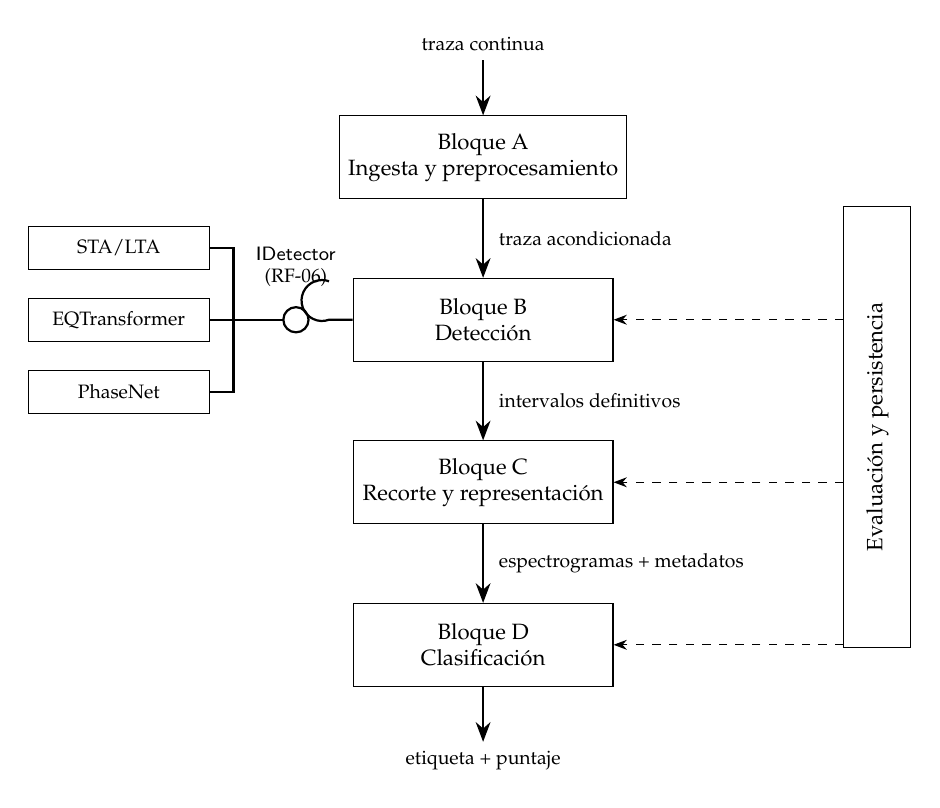
\begin{tikzpicture}[
  font=\footnotesize,
  bloque/.style={draw, rectangle, align=center, minimum height=1.05cm,
    minimum width=3.3cm, inner sep=3pt},
  sub/.style={draw, rectangle, align=center, inner sep=2.5pt,
    font=\scriptsize, minimum width=2.3cm, minimum height=0.55cm},
  flujo/.style={-{Stealth[length=2.5mm]}, thick},
  etiq/.style={font=\scriptsize, align=left},
  >=Stealth]
% Cadena principal, vertical
\node[bloque] (A) {Bloque A\\Ingesta y preprocesamiento};
\node[bloque, below=1.0cm of A] (B) {Bloque B\\Detección};
\node[bloque, below=1.0cm of B] (C) {Bloque C\\Recorte y representación};
\node[bloque, below=1.0cm of C] (D) {Bloque D\\Clasificación};
% Flechas de la cadena con el dato que fluye
\node[above=0.7cm of A, etiq, align=center] (traza) {traza continua};
\draw[flujo] (traza) -- (A);
\draw[flujo] (A) -- node[etiq, right=2pt] {traza acondicionada} (B);
\draw[flujo] (B) -- node[etiq, right=2pt] {intervalos definitivos} (C);
\draw[flujo] (C) -- node[etiq, right=2pt] {espectrogramas + metadatos} (D);
\node[below=0.7cm of D, etiq, align=center] (out) {etiqueta + puntaje};
\draw[flujo] (D) -- (out);
% Interfaz IDetector: la bola la proveen los detectores, la copa la
% requiere el envoltorio del bloque B
\coordinate (ifz) at ($(B.west)+(-0.72,0)$);
\draw[thick] (ifz) circle (1.6mm);
\node[etiq, above=3mm of ifz, align=center] {\textsf{IDetector}\\(RF-06)};
% Copa (interfaz requerida) desde el bloque B, abrazando la bola
\draw[thick] (B.west) -- ($(ifz)+(0.42,0)$)
  arc[start angle=-70, end angle=-290, radius=2.6mm];
% Detectores intercambiables, columna a la izquierda: proveen la bola
\node[sub] (eqt) at ($(ifz)+(-2.25,0)$) {EQTransformer};
\node[sub, above=0.35cm of eqt] (sta) {STA/LTA};
\node[sub, below=0.35cm of eqt] (pn) {PhaseNet};
\coordinate (junta) at ($(ifz)+(-0.75,0)$);
\draw[thick] (eqt.east) -- (junta);
\draw[thick] (sta.east) -- ++(0.30,0) |- (junta);
\draw[thick] (pn.east)  -- ++(0.30,0) |- (junta);
\draw[thick] (junta) -- ($(ifz)+(-0.16,0)$);
% Componente transversal de evaluacion, a la derecha
\node[bloque, rotate=90, minimum width=5.6cm, minimum height=0.85cm]
  (ev) at ($(C.east)+(3.35,0.7)$) {Evaluación y persistencia};
\draw[dashed, ->] (ev.north |- B.east) -- (B.east);
\draw[dashed, ->] (ev.north |- C.east) -- (C.east);
\draw[dashed, ->] (ev.north |- D.east) -- (D.east);
\end{tikzpicture}
\caption{Diagrama de componentes de la cadena de procesamiento. Los tres
detectores son intercambiables tras la interfaz \textsf{IDetector}; el
componente de evaluación observa las salidas de los bloques B, C y D sin
pertenecer a la cadena.}
\label{fig:arquitectura}
\end{figure}

El Cuadro~\ref{tab:rf-componente} indica el punto exacto de la arquitectura
donde se aplica cada requerimiento funcional, según exige el criterio de
aceptación de esta tarea de diseño.

{\small
\begin{longtable}{>{\raggedright\arraybackslash}p{4.6cm}>{\raggedright\arraybackslash}p{6.7cm}}
\caption{Asignación de requerimientos a los componentes de la arquitectura.}\label{tab:rf-componente}\\
\toprule
\textbf{Componente} & \textbf{Requerimientos que materializa} \\
\midrule
\endfirsthead
\multicolumn{2}{l}{\itshape Cuadro \thetable{} (continuación)}\\
\toprule
\textbf{Componente} & \textbf{Requerimientos que materializa} \\
\midrule
\endhead
\midrule
\multicolumn{2}{r}{\itshape Continúa en la página siguiente}\\
\endfoot
\bottomrule
\endlastfoot
Bloque A, ingesta y preprocesamiento & RF-01, RF-02, RF-03, RF-04, RF-05 \\
\addlinespace
Bloque B, envoltorio de barrido y fusión & RF-07, RF-08 y la fusión de
intervalos de la Sección~\ref{sec:recorte-espectrogramas} \\
\addlinespace
Bloque B, interfaz \textsf{IDetector} y detectores & RF-06; la
intercambiabilidad materializa RNF-04 \\
\addlinespace
Bloque C, recorte y representación & RF-09, RF-10, RF-11, RF-12, RF-13 \\
\addlinespace
Bloque D, clasificación & RF-14, RF-15, RF-16, RF-17 \\
\addlinespace
Evaluación y persistencia & RF-18, RF-19, RF-20; RNF-08 \\
\end{longtable}
}

\section{Contrato de datos entre bloques}
\label{sec:contrato-datos}

Cada conector de la Figura~\ref{fig:arquitectura} transporta una estructura
con campos, tipos y unidades fijos. Especificarlos por separado del código
persigue un objetivo concreto: que cualquiera de los cuatro bloques pueda
reimplementarse leyendo solo este contrato, sin inspeccionar la
implementación del bloque anterior. Tres convenciones rigen los tres
conectores.

La primera es la representación del tiempo. Toda referencia temporal viaja
por duplicado: como índice de muestra, entero, y como marca de tiempo Unix en
segundos. El índice de muestra es la referencia canónica y el tiempo Unix es
derivado, porque la traza continua concatena tres segmentos de fechas no
consecutivas, según se detalla en el Cuadro~\ref{tab:tramos}: el
índice crece de forma continua a lo largo del archivo, mientras que la marca
de tiempo salta en las muestras 2.160.000 y 3.240.001. Toda aritmética de
duración y de solapamiento se realiza sobre índices; el tiempo Unix se emplea
únicamente para reportar. Como salvaguarda, cada estructura declara el
identificador del bloque temporal al que pertenece, y ningún intervalo puede
declarar índices de dos bloques distintos.

La segunda es el puntaje de detección. STA/LTA entrega una razón de energía
no acotada superiormente, mientras que los detectores profundos entregan
probabilidades en el intervalo unitario. El contrato transporta ambos: el
puntaje crudo tal como lo produce el detector y el puntaje normalizado al
intervalo unitario mediante la transformación declarada por cada
implementación. Declaro la limitación que esto impone: el puntaje normalizado
permite ordenar detecciones dentro de un mismo detector, pero no es
comparable entre detectores, y ninguna decisión del sistema puede apoyarse en
esa comparación.

La tercera es la procedencia. Cada estructura arrastra el identificador del
detector o del modelo que la produjo y el de la configuración empleada, de
modo que cualquier cifra reportada pueda regenerarse desde el registro
almacenado, según exige RF-20.

El detalle campo por campo de los tres conectores, con su tipo, su unidad y
su restricción de validez, está en el Anexo~\ref{sec:anexo-contrato}.

La salida del bloque D agrega al registro del último conector el vector de
cuatro puntajes, uno por clase VT, LP, TR y rechazo, la etiqueta de máximo puntaje y
el identificador del modelo empleado. Ese registro completo es la unidad que
el componente de evaluación persiste y que alimenta el archivo tabular de
inspección exigido por RNF-08.

Dos reglas de validación acompañan al contrato y se comprobarán con casos
sintéticos antes de conectar bloques reales: ninguna estructura puede declarar
índices pertenecientes a dos bloques temporales distintos, y todo campo
derivado, como \texttt{duracion} o \texttt{tiempo\_inicio}, debe poder
recalcularse desde los índices y la frecuencia sin discrepancia.

\section{Interfaz común de detección}
\label{sec:interfaz-deteccion}

La interfaz \textsf{IDetector} es la que permite sustituir el detector sin
modificar el resto de la cadena, según exige RNF-04, y la que hace posible que
la variabilidad del recorte entre detectores sea el objeto de estudio y no un
obstáculo. La especifico sin referencia a ningún detector concreto: describe
qué debe entregar una implementación, no cómo obtenerlo.

El reparto de responsabilidades es la decisión central. Una implementación de
\textsf{IDetector} resuelve únicamente la detección local sobre el fragmento
de traza que recibe. Todo lo demás vive en el envoltorio de barrido del
bloque B: el recorrido con ventanas de 300\,s, la expansión de arribo a
intervalo, la fusión de detecciones en bordes de ventana y el ensamblado del
registro que exige el contrato de datos. Concentrar esa lógica fuera de los
detectores es lo que evita reimplementarla tres veces y lo que garantiza que
los tres se evalúen bajo el mismo criterio.

La interfaz declara cuatro operaciones. \texttt{describir} entrega los
metadatos de la implementación: su identificador, su versión y dos
declaraciones de capacidad que el envoltorio necesita conocer de antemano, a
saber, si el detector delimita eventos o solo entrega arribos, y cuántas
componentes exige su entrada. \texttt{configurar} recibe los parámetros
propios del detector y devuelve el identificador de configuración que el
contrato de datos arrastra hasta la salida. \texttt{detectar} recibe un
fragmento de traza acondicionada y devuelve la lista de detecciones locales,
cada una con su índice de inicio, su índice de término cuando el detector
delimita, su índice de arribo cuando no lo hace, y su puntaje crudo.
\texttt{normalizar\_puntaje} convierte el puntaje crudo al intervalo unitario
mediante la transformación propia de cada implementación, que es la única
forma de reconciliar una razón de energía no acotada con una probabilidad.

Las dos declaraciones de capacidad no son adornos: determinan el
comportamiento del envoltorio. Si la implementación declara que no delimita,
el envoltorio aplica la regla de expansión de arribo a intervalo (RF-07) y
marca el resultado como \texttt{expandido} en el contrato. Si declara que
exige tres componentes, el bloque A aplica la estrategia de relleno declarada
para ese modelo (RF-03), cuyo efecto sobre el techo de recall quedó medido en
E8. Así, las dos particularidades que diferencian a los detectores evaluados
quedan resueltas por declaración y no por casos especiales dentro del código
del envoltorio.

El Cuadro~\ref{tab:idetector} del Anexo~\ref{sec:anexo-contrato} demuestra
que los tres detectores evaluados encajan en la interfaz sin excepciones, que
es el criterio de aceptación de esta tarea de diseño. Incluye además el
detector sintético con el que se validará la implementación: al producir
intervalos conocidos de antemano, permite comprobar que la cadena entrega
exactamente lo esperado antes de conectar un detector real, según la
definición de terminado del backlog.


Declaro una consecuencia de este diseño que conviene no ocultar. La interfaz
uniforma la forma de la salida, no su significado: el puntaje normalizado de
STA/LTA y el de EQTransformer son ambos números en el intervalo unitario, pero
no miden lo mismo, de modo que la comparación entre detectores debe hacerse
sobre métricas de desempeño y nunca sobre sus puntajes, tal como se estableció
en la Sección~\ref{sec:contrato-datos}.

\section{Procedimiento de recorte adaptativo y generación de espectrogramas}
\label{sec:recorte-espectrogramas}

El procedimiento resuelve la tensión identificada en E5: los detectores y el
clasificador exigen entradas de extensión acotada, mientras que las duraciones
observadas van de 3,4\,s a 240,8\,s y la mediana de TR excede la ventana fija
de 81,92\,s. Lo diseño en tres etapas encadenadas: barrido, fusión y recorte.

\textbf{Barrido con traslape.} Recorreré la traza continua con ventanas de
análisis de 300\,s y paso de 55\,s. La ventana supera la duración máxima
observada en el catálogo (240,8\,s) y el paso cumple la condición
$paso \leq ventana - d_{\max} = 59{,}2$\,s, de modo que, por construcción, todo
evento del rango observado queda contenido completo en al menos una ventana.
La ventana de barrido es la unidad de entrega al detector, no la unidad de
análisis: STA/LTA calcula su estadístico muestra a muestra, y los detectores
profundos segmentan internamente la entrada en sus tramos nativos, por lo que
ampliar la ventana de barrido no altera la detectabilidad de los eventos
cortos. Sobre la traza de 10,18\,horas el barrido produce cerca de 660
ventanas, ejecutables en CPU.

\textbf{Fusión de intervalos.} Cuando una detección alcance el borde derecho
de su ventana, buscaré su continuación en la ventana siguiente y fusionaré
ambos intervalos si se solapan temporalmente o si su separación es inferior a
un umbral declarado. Con el paso elegido la fusión actúa como red de
seguridad, no como mecanismo principal: la condición del paso ya garantiza
una ventana que contiene el evento entero.

\textbf{Recorte y espectrograma.} El clasificador nunca recibe la ventana de
barrido. Para cada intervalo fusionado recortaré la traza con duración
adaptada al intervalo, más un margen de contexto previo que tolere el error
de onset medido (1,7\,s a 2,4\,s, E9), y generaré desde ese recorte el
espectrograma de dimensiones fijas. Así un evento de 3,4\,s y uno de 240,8\,s
ocupan por igual la representación de entrada, y la información de duración
se reinyecta de forma explícita según lo exige RF-13.

\textbf{Normalización.} La amplitud no se normalizará a nivel de ventana de
barrido: si en una misma ventana coinciden un evento extenso de gran amplitud
y uno breve de amplitud baja, la normalización conjunta aplastaría al segundo.
Cada detector conservará la normalización de su tramo nativo y la
normalización del espectrograma se aplicará por recorte individual.

\textbf{Validación con casos sintéticos.} Antes de aplicar el procedimiento a
datos reales, lo validaré con tres casos de solución conocida, según exige
RF-12: un evento de 3,4\,s aislado en una ventana de 300\,s, que debe
detectarse con el mismo onset que en la configuración de ventana fija; un
evento de 240,8\,s que cruza el borde entre dos ventanas consecutivas, que la
fusión debe recuperar entero; y un evento breve de amplitud baja a 30\,s de un
evento extenso de amplitud diez veces mayor dentro de la misma ventana, que
deben resolverse como intervalos separados. Si el tercer caso falla, el
diagnóstico apunta a la normalización y no al umbral de detección.

Este procedimiento garantiza que ningún evento se pierda por truncamiento ni
por borde de ventana. No garantiza que todo evento sea detectado: el recall
medido de los detectores (0,542 a 0,581) es una propiedad de los modelos, no
del recorte, y su relación con la razón señal-ruido de los eventos no
detectados se analizará por separado. Las detecciones de clases no volcánicas
no se filtran en esta etapa: llegan al clasificador y es la clase de rechazo
(RF-14) la que las resuelve, según lo medido en E6.

\section{Clasificador por transferencia de aprendizaje}
\label{sec:clasificador-transferencia}

Desarrollaré esta sección en el sprint 3, junto con la tarea B-23, que ajusta
la VGG16 preentrenada en ImageNet a las cuatro clases de salida bajo el
protocolo común de entrenamiento y evaluación.

\section{Protocolo de evaluación integrada}
\label{sec:protocolo-evaluacion}

Desarrollaré esta sección en el sprint 3, junto con las tareas B-25, que mide
el tiempo de procesamiento de la cadena completa en CPU, y B-26, que compara
la clasificación sobre recortes de referencia y automáticos con intervalos
de confianza.

% ======================================================================
% CAPITULO 3. Estrategia y resultados de los detectores (OE1)
% ======================================================================
\chapter{Estrategia y resultados de los detectores}
\label{cap:detectores}

% Pendiente: parrafo de entrada. Este capitulo responde a OE1 y al pedido del
% 21-09 de mostrar esquema, descripcion y desempeno de cada detector.

\section{Datos de evaluación}
\label{sec:datos-evaluacion}

Evalúo los detectores sobre la traza continua de diez horas del conjunto de
datos de Zenodo, que concatena tres tramos de fechas no consecutivas. El
Cuadro~\ref{tab:tramos} muestra, para cada tramo, su posición en la traza y su
hora de inicio y término. Las horas provienen de los nombres de los archivos
crudos que el profesor guía compartió el 22 de septiembre de 2026, que
codifican en tiempo Unix el inicio y el término de cada tramo, y coinciden con
las fechas de la fila de tiempo de la traza. En las tres fechas regía en Chile
el horario de verano, de modo que la hora local es la UTC menos tres horas; el
tramo 2 comienza, en hora local, la noche del 13 de enero de 2020.

{\small
\begin{longtable}{>{\centering\arraybackslash}p{1.2cm}>{\raggedleft\arraybackslash}p{1.7cm}>{\raggedleft\arraybackslash}p{1.7cm}>{\centering\arraybackslash}p{1.9cm}>{\centering\arraybackslash}p{1.6cm}>{\centering\arraybackslash}p{1.6cm}}
\caption{Tramos de la traza continua de evaluación, con su hora de inicio y término en UTC.}\label{tab:tramos}\\
\toprule
\textbf{Tramo} & \textbf{Muestra inicial} & \textbf{Muestras} & \textbf{Fecha} & \textbf{Inicio} & \textbf{Término} \\
\midrule
\endfirsthead
\multicolumn{6}{l}{\itshape Cuadro \thetable{} (continuación)}\\
\toprule
\textbf{Tramo} & \textbf{Muestra inicial} & \textbf{Muestras} & \textbf{Fecha} & \textbf{Inicio} & \textbf{Término} \\
\midrule
\endhead
\midrule
\multicolumn{6}{r}{\itshape Continúa en la página siguiente}\\
\endfoot
\bottomrule
\endlastfoot
1 & 0 & 2.160.000 & 2018-02-09 & 04:06:58 & 10:06:58 \\
2 & 2.160.000 & 1.080.001 & 2020-01-14 & 01:06:58 & 04:06:58 \\
3 & 3.240.001 & 424.192 & 2017-01-10 & 06:06:58 & 07:17:40 \\
\end{longtable}
}

A 100~Hz, la duración nominal de cada tramo corresponde a 2.160.000, 1.080.000
y 424.200 muestras. Los tramos 2 y 3 de la traza difieren de ese valor en una
muestra de más y ocho de menos, respectivamente. Por esa diferencia no asumiré
que la traza y los archivos crudos están alineados muestra a muestra: mediré la
alineación antes de usar los archivos crudos. Según el profesor guía, la traza
de Zenodo equivale a esos archivos filtrados con un pasabanda Butterworth de
orden 5 entre 1 y 15~Hz, aplicado en fase cero; los archivos crudos no traen
ese filtro. Verificaré esa equivalencia filtrando los archivos crudos y
comparándolos canal por canal con la traza antes de emplearlos.

\section{STA/LTA}
\label{sec:det-stalta}
% Pendiente: esquema, descripcion y resultados en los dos niveles.

\section{EQTransformer}
\label{sec:det-eqt}
% Pendiente: esquema, descripcion y resultados en los dos niveles.

\section{PhaseNet}
\label{sec:det-phasenet}
% Pendiente: esquema, descripcion y resultados de nivel 1. No delimita
% eventos, solo entrega arribos P y S; su exclusion del nivel 2 es un
% resultado.

\section{Comparación y criterio de operación}
\label{sec:det-comparacion}
% Pendiente: comparacion global y por clase, y situacion frente al criterio
% de sensibilidad de 0,95 con la menor tasa de falsos positivos.

% ======================================================================
% CAPITULO 4. Registro de avance del backlog (rubrica: 10 % y 15 %)
% ======================================================================
\chapter{Registro de avance del backlog}
\label{cap:registro}

\section{Tareas de diseño del sprint 1}
\label{sec:esfuerzo}
% Pendiente: horas reales de B-04, B-05, B-06 y B-08 (estimadas 6, 6, 5 y 6)
% contra el backlog completo.

\section{Desviaciones y tareas nuevas}
\label{sec:desviaciones}
% Pendiente: B-01 postergada, estado de B-05 y tareas nuevas del 21-09
% (barrido hacia sensibilidad de 0,95, razon senal-ruido, desglose por tramo,
% implementacion de las ventanas de 5 minutos).

\section{Repositorio y registro de commits}
\label{sec:repositorio}

El código y las fuentes de este informe se versionan en el repositorio público
\url{https://github.com/Pattoxd45/tesis-sismovolcanica}, rama \texttt{main}.
El Cuadro~\ref{tab:commits} lista los commits de esta etapa, con la tarea del
backlog a la que responde cada uno y la sección del informe donde se refleja.

{\small
\begin{longtable}{>{\raggedright\arraybackslash}p{1.5cm}>{\raggedright\arraybackslash}p{1.9cm}>{\raggedright\arraybackslash}p{1.6cm}>{\raggedright\arraybackslash}p{5.6cm}}
\caption{Commits de la Etapa 2 en el repositorio del proyecto.}\label{tab:commits}\\
\toprule
\textbf{Commit} & \textbf{Fecha} & \textbf{Tarea} & \textbf{Contenido} \\
\midrule
\endfirsthead
\multicolumn{4}{l}{\itshape Cuadro \thetable{} (continuación)}\\
\toprule
\textbf{Commit} & \textbf{Fecha} & \textbf{Tarea} & \textbf{Contenido} \\
\midrule
\endhead
\midrule
\multicolumn{4}{r}{\itshape Continúa en la página siguiente}\\
\endfoot
\bottomrule
\endlastfoot
\texttt{8d7c709} & 2026-09-18 & --- &
Incorpora la retroalimentación del 15 de septiembre: objetivos reformulados y
sus consecuencias en requerimientos, alternativas y backlog
(Sección~\ref{sec:objetivos-reformulados}) \\
\addlinespace
\texttt{6648b5f} & 2026-09-18 & B-08 &
Procedimiento de barrido con ventanas de 300~s, fusión y recorte adaptativo
(Sección~\ref{sec:recorte-espectrogramas}) \\
\addlinespace
\texttt{f25e071} & 2026-09-18 & B-04 &
Diagrama de componentes UML de la cadena de procesamiento
(Sección~\ref{sec:arquitectura-cadena}) \\
\addlinespace
\texttt{98ebf4c} & 2026-09-19 & B-05 &
Contrato de datos entre bloques (Sección~\ref{sec:contrato-datos} y
Anexo~\ref{sec:anexo-contrato}) \\
\addlinespace
\texttt{0377d0b} & 2026-09-30 & B-06 &
Interfaz común de detección \texttt{IDetector}
(Sección~\ref{sec:interfaz-deteccion}) \\
% Agregar aqui el commit de este informe y los que sigan.
\end{longtable}
}

% Sin efecto mientras el informe no tenga citas.
\printbibliography

\appendix
\chapter{Anexos}
\label{cap:anexos}

\section{Contrato de datos entre bloques}
\label{sec:anexo-contrato}

Se especifican aquí los tres conectores de la cadena descritos en la
Sección~\ref{sec:contrato-datos}, con el nombre, el tipo, la unidad y la
restricción de cada campo. El detalle es suficiente para reimplementar
cualquier bloque sin inspeccionar la implementación del anterior.

{\small
\begin{longtable}{>{\raggedright\arraybackslash}p{2.9cm}>{\raggedright\arraybackslash}p{2.5cm}>{\raggedright\arraybackslash}p{5.9cm}}
\caption{Contrato del conector A\,$\rightarrow$\,B, traza acondicionada.}\label{tab:contrato-ab}\\
\toprule
\textbf{Campo} & \textbf{Tipo y unidad} & \textbf{Significado y restricción} \\
\midrule
\endfirsthead
\multicolumn{3}{l}{\itshape Cuadro \thetable{} (continuación)}\\
\toprule
\textbf{Campo} & \textbf{Tipo y unidad} & \textbf{Significado y restricción} \\
\midrule
\endhead
\midrule
\multicolumn{3}{r}{\itshape Continúa en la página siguiente}\\
\endfoot
\bottomrule
\endlastfoot
\texttt{datos} & arreglo real, cuentas & Matriz de $c \times n$ muestras, con
$c$ componentes y $n$ muestras. Sin normalizar \\
\addlinespace
\texttt{frecuencia} & real, Hz & Frecuencia de muestreo, 100 en todos los
casos \\
\addlinespace
\texttt{canal} & entero & Fila de origen en el archivo, restringida a los
canales utilizables 1, 2, 3, 5 y 6 \\
\addlinespace
\texttt{bloque} & entero & Segmento temporal de procedencia, 1 a 3 \\
\addlinespace
\texttt{muestra\_inicial} & entero & Índice de la primera muestra respecto del
archivo completo \\
\addlinespace
\texttt{tiempo\_inicial} & real, s & Marca de tiempo Unix de la primera
muestra, derivada de la fila 0 \\
\addlinespace
\texttt{relleno} & cadena & Estrategia de relleno de componentes aplicada
(RF-03); \texttt{ninguno} cuando el detector opera sobre un solo canal \\
\end{longtable}
}

{\small
\begin{longtable}{>{\raggedright\arraybackslash}p{2.9cm}>{\raggedright\arraybackslash}p{2.5cm}>{\raggedright\arraybackslash}p{5.9cm}}
\caption{Contrato del conector B\,$\rightarrow$\,C, intervalos definitivos.}\label{tab:contrato-bc}\\
\toprule
\textbf{Campo} & \textbf{Tipo y unidad} & \textbf{Significado y restricción} \\
\midrule
\endfirsthead
\multicolumn{3}{l}{\itshape Cuadro \thetable{} (continuación)}\\
\toprule
\textbf{Campo} & \textbf{Tipo y unidad} & \textbf{Significado y restricción} \\
\midrule
\endhead
\midrule
\multicolumn{3}{r}{\itshape Continúa en la página siguiente}\\
\endfoot
\bottomrule
\endlastfoot
\texttt{id} & cadena & Identificador único de la detección dentro de la
ejecución \\
\addlinespace
\texttt{muestra\_inicio} & entero & Índice de inicio del intervalo \\
\addlinespace
\texttt{muestra\_fin} & entero & Índice de término; debe cumplir
\texttt{muestra\_fin} $>$ \texttt{muestra\_inicio} y pertenecer al mismo
bloque \\
\addlinespace
\texttt{tiempo\_inicio} & real, s & Marca Unix derivada del índice de inicio \\
\addlinespace
\texttt{duracion} & real, s & Diferencia de índices dividida por la frecuencia;
campo derivado, incluido por conveniencia de lectura \\
\addlinespace
\texttt{canal}, \texttt{bloque} & entero & Heredados de la traza de origen \\
\addlinespace
\texttt{puntaje\_crudo} & real & Valor tal como lo entrega el detector, sin
acotar \\
\addlinespace
\texttt{puntaje} & real, $[0,1]$ & Puntaje normalizado; comparable solo dentro
de un mismo detector \\
\addlinespace
\texttt{detector} & cadena & Identificador del detector que produjo la
detección \\
\addlinespace
\texttt{config} & cadena & Identificador de la configuración empleada, para
RF-20 \\
\addlinespace
\texttt{origen\_intervalo} & cadena & \texttt{directo} cuando el detector
delimita, \texttt{expandido} cuando se aplicó la regla de expansión de arribo
(RF-07) \\
\addlinespace
\texttt{fusionado} & booleano & Verdadero si el intervalo resulta de fusionar
detecciones de ventanas de barrido contiguas \\
\end{longtable}
}

{\small
\begin{longtable}{>{\raggedright\arraybackslash}p{2.9cm}>{\raggedright\arraybackslash}p{2.5cm}>{\raggedright\arraybackslash}p{5.9cm}}
\caption{Contrato del conector C\,$\rightarrow$\,D, espectrogramas y metadatos.}\label{tab:contrato-cd}\\
\toprule
\textbf{Campo} & \textbf{Tipo y unidad} & \textbf{Significado y restricción} \\
\midrule
\endfirsthead
\multicolumn{3}{l}{\itshape Cuadro \thetable{} (continuación)}\\
\toprule
\textbf{Campo} & \textbf{Tipo y unidad} & \textbf{Significado y restricción} \\
\midrule
\endhead
\midrule
\multicolumn{3}{r}{\itshape Continúa en la página siguiente}\\
\endfoot
\bottomrule
\endlastfoot
\texttt{id} & cadena & Heredado del intervalo que originó el recorte \\
\addlinespace
\texttt{espectrograma} & arreglo real & Matriz de dimensiones fijas,
frecuencia por tiempo, idénticas para todo evento \\
\addlinespace
\texttt{duracion\_real} & real, s & Duración del recorte antes de llevarlo a
dimensiones fijas; es la información que RF-13 exige preservar de forma
explícita \\
\addlinespace
\texttt{margen\_previo} & real, s & Contexto antepuesto al inicio estimado
para tolerar el error de onset (RF-11) \\
\addlinespace
\texttt{truncado} & booleano & Verdadero si se aplicó la política para
eventos que exceden la ventana nominal (RF-10) \\
\addlinespace
\texttt{solapa\_con} & lista de cadenas & Identificadores de detecciones
cuyo intervalo se solapa con este, tras aplicar la regla de resolución
(RF-12); lista vacía en el caso habitual \\
\addlinespace
\texttt{normalizacion} & cadena & Procedimiento de normalización aplicado al
recorte individual \\
\addlinespace
\texttt{detector}, \texttt{config}, \texttt{canal}, \texttt{bloque} & cadena y
entero & Heredados del intervalo, para conservar la procedencia hasta la
salida \\
\end{longtable}
}



{\small
\begin{longtable}{>{\raggedright\arraybackslash}p{2.4cm}>{\raggedright\arraybackslash}p{1.6cm}>{\raggedright\arraybackslash}p{1.6cm}>{\raggedright\arraybackslash}p{5.3cm}}
\caption{Encaje de los detectores evaluados en la interfaz \textsf{IDetector}.}\label{tab:idetector}\\
\toprule
\textbf{Implementación} & \textbf{Delimita} & \textbf{Compon.} & \textbf{Puntaje crudo y su normalización} \\
\midrule
\endfirsthead
\multicolumn{4}{l}{\itshape Cuadro \thetable{} (continuación)}\\
\toprule
\textbf{Implementación} & \textbf{Delimita} & \textbf{Compon.} & \textbf{Puntaje crudo y su normalización} \\
\midrule
\endhead
\midrule
\multicolumn{4}{r}{\itshape Continúa en la página siguiente}\\
\endfoot
\bottomrule
\endlastfoot
STA/LTA & Sí & 1 & Razón de energía, no acotada superiormente; se normaliza
respecto del umbral de disparo configurado \\
\addlinespace
EQTransformer & Sí & 3 & Probabilidad de detección en $[0,1]$; la
normalización es la identidad \\
\addlinespace
PhaseNet & No & 3 & Probabilidad de arribo en $[0,1]$; la normalización es la
identidad y el envoltorio expande el arribo a intervalo \\
\addlinespace
Detector sintético & Sí & 1 & Puntaje fijo declarado en el caso de prueba;
la normalización es la identidad \\
\end{longtable}
}

\end{document}
